\documentclass[twocolumn]{article} 
\usepackage{graphicx}
\usepackage[margin=2.0cm]{geometry} % Decrease margin size
\usepackage{xcolor}
\usepackage{float}
\usepackage{xcolor}
\usepackage[hyphens,spaces,obeyspaces]{url}
\usepackage[numbers]{natbib}
\usepackage{listings}
\usepackage{subcaption}
\usepackage{lipsum}
\usepackage{tikz}
\usetikzlibrary{positioning}
\usetikzlibrary{graphs,graphs.standard}
% Define grayscale colors
\definecolor{codegray}{gray}{0.95} % Background color
\definecolor{codeblack}{gray}{0.1} % Text color
\definecolor{codecomment}{gray}{0.5} % Comment color

% Define custom lstlisting style
\lstdefinestyle{researchpaper}{
    backgroundcolor=\color{codegray},
    basicstyle=\ttfamily\small\color{codeblack},
    commentstyle=\color{codecomment},
    frame=single,
    framerule=0pt,
    rulecolor=\color{codeblack},
    aboveskip=10pt,
    belowskip=10pt,
    showstringspaces=false,
    breaklines=true,
    breakatwhitespace=true,
    captionpos=b,
    numbersep=5pt,
    numberstyle=\tiny\color{codeblack},
}

\usepackage{amsmath}
\usepackage{amsfonts}
\usepackage{fancyhdr}
% Header
\pagestyle{fancy}
\fancyhf{} % Clear all header and footer fields
\lhead{\nouppercase{\leftmark}} % Left align section title in header
\rhead{\nouppercase{\rightmark}} % Right align subsection title in header
\cfoot{\thepage} % Center align page number in footer

% Header
\renewcommand{\headrulewidth}{0.2pt} % Set the thickness of the header line
\renewcommand{\footrulewidth}{0.2pt} % Set the thickness of the footer line

% Footer
\fancyfoot{} % Clear footer fields
\lfoot{\today} % Left align current date in footer
\cfoot{} % Center align nothing in footer
\rfoot{Zewail City of Science and Technology} % Right align university name in footer

\title{Discrete Mathematics (MATH 308) - Spring 2024 \\ Course Project - Pathfinding Simulation }
\author{Saifelden Mohamed 202100432\\
Aser Osama 202101266\\
Omar Elsayed 202100597\\}
\date{}

\makeatletter
\renewcommand{\maketitle}{
    \thispagestyle{empty} % Remove header and footer from this page
    \vspace*{\fill} % Vertically center content
    \begin{center}
        {\huge\@title}
        
        \vspace{1cm}
        \includegraphics[width=0.5\textwidth]{zew.png}
        
        \vspace{0.5cm}

        \Large

        \begin{tabular}{c}
            \@author
        \end{tabular}

        \vspace{0.5cm}

        
        \Large
        Communications and Information Engineering\\
        Zewail City of Science and Technology\\
        \Large
        \today
    \end{center}
    \vspace*{\fill} % Vertically center content
}
\makeatother
\begin{document}

\onecolumn % Switch to one column layout
\maketitle
\thispagestyle{empty} % Remove page number from title page

\newpage
\tableofcontents

\newpage
\twocolumn 

\section{Introduction}
Path Finding Algorithms are of crucial importance in today’s world. As it can be applied in Navigation systems, algorithms like A* and Dijkstra can find the shortest path for navigation in road networks to traverse a city efficiently. It can also be used in Navigation for Robotics to find the shortest path between two points avoiding obstacles. As there exists a competition called the Maze Solver challenge is based on the least time a robot mouse can traverse a maze, which involves finding the shortest path on the spot during the competition. 

Another application is in game development, as character movement in games should traverse the shortest path having the least obstacles. Path-finding algorithms can also be applied in Network routing for different networking topologies as in Internet traffic data packets are demanded to traverse the faster routes to the client machine from the server in a formidable manner for faster service. As well as telecommunications for a communication system, the source and receiver would need to traverse the fastest route through the communication network composed of intermediate receivers, processors, and antennas in case of wireless communication to ensure better and faster service with less attenuation and less power loss. 

Each of these systems can be modeled as either a directed on the undirected graph, simple or non-simple, weighted or unweighted. The A* (A-star) was originally developed by Peter Hart, Nils Nilsson, and Bertram Raphael in 1968. As the A* algorithm uses both the strengths of the Dijkstra algorithm and the Best-First Search Algorithm. A* fundamentally different from the Dijkstra in its heuristic approach to the path-finding problem. This primarily reduces the number of nodes that need to be searched in order to reach the shortest path between two points in optimal conditions in a given graph. It works by maintaining a priority queue of paths, scored by a cost function that combines the distance from the start node with an estimated distance to the goal node. 

The heuristic approach allows A* to navigate through complex and large spaces as it’s useful especially in game development and robotics as we have listed in the applications above. The algorithm is used primarily as a cornerstone in the fields of artificial intelligence and operations research with a complexity of $O(b^d)$ as b is a branching factor and d is the number of nodes in the given graph. Dijkstra’s Algorithm on the other hand is named after the Dutch computer scientist Edsger W. Dijkstra. As it’s made before the A* algorithm, it presents a fundamental building block in graph theory and computer science as it’s one of the first efficient shortest path algorithms used in computing. It operates by iteratively expanding the shortest path with each node traversed in the graph to a consistent distance weight-comparison from one node to the following one updating the path of the shortest distance until it reaches the goal node. 

The complexity of the Dijkstra algorithm is $O(V^2)$ as V is the number of vertices and $O((V+E)logV)$ when implemented with a priority queue data structure. In our project, we would write a path-finding program using the A and Dijkstra’s algorithm to find the shortest path in weighted simple graphs.
\section{Methodology}
We have written a program to illustrate the differences between the heuristic approach and the standard mathematical approach. The program reads the Graph map from a text file and runs through one of two algorithms to find the shortest path. The algorithms we have chosen to focus on for this simulation is A* and Djiskestra. However, in order to understand the following implementation, one needs to be briefed on the pixel grid represantation of a the standard Discrete Maths graph.
\subsection{Theoretical}
In Figure~\ref{fig:test}, you can see an example of the pixel grid analogy with the discrete maths graph. Each pixel is equivalent to a node that is connected to each pixel adjacent to it as well as each pixel diagonal to it. We assume the diagonal connections have larger weight than the adjacent connections. We used the following Analogy to generate the simulation we will use to test both Djikestra and A* to make any possible observations on them.
\begin{figure}[H]
    \centering
    \begin{subfigure}{0.235\textwidth}
        \centering
        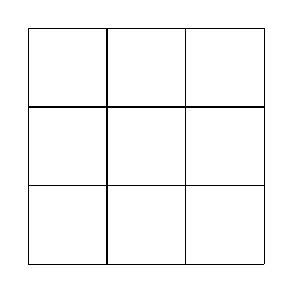
\begin{tikzpicture}
            \draw (0,0) grid (3,3);
        \end{tikzpicture}
        \caption{Pixel Grid}
    \end{subfigure}
    \hfill
    \begin{subfigure}{0.235\textwidth}
        \centering
          \includegraphics[width=0.8\textwidth]{figures/graph.png}
        \caption{Equivalent Graph}
    \end{subfigure}
    \caption{Pixel Grid Graph Representation}
    \label{fig:test}
\end{figure}
The pseudocode used for both algorithms is present in Listing~\ref{lst:Djikestra} and Listing~\ref{lst:A}. 
Djikestra's algorithm is a foundational method for solving the shortest path problem. It operates on the principle of iteratively exploring all of the vertices to determine the shortest path from a designated source vertex to all other vertices in a weighted graph. It initially sets all of it's weights to infinity except for the source vertex. Through iteratively selecting the vertices with the minimum distances from the source it updates the distances to it's neighbors if a shorter path is found. This process continues, like said earlier, until it has covered all vertices. Though optimality is guaranteed, this may not be the quickest way to find the shortest path and as we will see in our computer simulation, it ends up flooding the graph during its search. Often looking in places where it need not look. 

A*, on the other hand is an extension of the Djikestra's approach that integrations a heuristic function into the search process. It combines advantages from the heuristic search with Djiskestra's. It maintians two critical metrics, the gScore and the fScore. The addition of the gScore and the hScore produces the fScore, which is the score it uses to make its deicions on. The gScore represents the actual cost or distance from the start node to the current node n along the path discovered so far. Mathematically, gScore[n] is defined as the cost of the cheapest path from the start node to node n currently known. During the algorithm's execution, the gScore values are continuously updated as the algorithm explores different paths. If a shorter path to a node is discovered, its gScore is updated accordingly. The fScore combines the gScore with an estimated cost to reach the goal from the current node n. It represents the algorithm's current best guess as to how cheap a path could be from the start node to the goal if it goes through node n. Mathematically, fScore[n] is calculated as the sum of gScore[n] and an estimated heuristic cost (h(n)) from node n to the goal. The heuristic function h(n) provides an optimistic estimate of the cost to reach the goal from node n. It guides the search by biasing exploration towards nodes that are closer to the goal, thus potentially leading to more efficient search and faster convergence towards the optimal path. Using these scores  It intelligently prioritizes exploration by favoring nodes that are likely to lead to the goal efficiently, guided by the heuristic function. This heuristic-guided search significantly reduces the search space, leading to faster convergence towards optimal solutions. By leveraging both the principles of Dijkstra's algorithm and heuristic search, A* algorithm offers an efficient and effective solution for finding optimal paths. 

In the following part we will test both Algorithms on multiple test cases and make some comments.

\subsection{Implementation}
Using the pixel graph implementation we ran the simulation which was written in C++ using the SFML library to render a simple GUI. The Purple node is the end position, the start position is the bottom right corner. The red nodes are nodes that are covered and the blue nodes indicate the final path. A thin black line outlines every pixel for clarity. The grid, start, and destination points are loaded from a file, and the algorithm to be used is specified in the file as well. The code continuously updates the visualization of the grid and the pathfinding process until the destination is reached or the window is closed.

\section{Results and Simulations}

\begin{figure}[H]
    \centering
    \begin{subfigure}{0.235\textwidth}
        \centering
        \includegraphics[width=0.8\textwidth]{figures/2024-05-22_22-44_1.png}
        \caption{Mid Simulation}
    \end{subfigure}
    \hfill
    \begin{subfigure}{0.235\textwidth}
        \centering
          \includegraphics[width=0.8\textwidth]{figures/2024-05-22_22-44.png}
        \caption{Final Path}
    \end{subfigure}
    \caption{Djikestra Algorithm}
    \label{fig:test2}
\end{figure}

In Figure~\ref{fig:test2}, we can make the observation that Djikestra is indeed covering nearly every node in order to find the final position producing this flooding effect we spoke of earlier.

\begin{figure}[H]
    \centering
    \begin{subfigure}{0.235\textwidth}
        \centering
        \includegraphics[width=0.8\textwidth]{figures/2024-05-22_22-45_1.png}
        \caption{Mid Simulation}
    \end{subfigure}
    \hfill
    \begin{subfigure}{0.235\textwidth}
        \centering
          \includegraphics[width=0.8\textwidth]{figures/2024-05-22_22-45.png}
        \caption{Final Path}
    \end{subfigure}
    \caption{A* Simulation}
    \label{fig:test3}
\end{figure}

In Figure~\ref{fig:test3}, We can view that far fewer nodes are covered for a relatively similar path allowing it to find the final point much more efficiently.

\section{Conclusion}
In conclusion, utilizing Dijkstra’s and A* algorithms for pathfinding techniques among simple weighted graphs has been an eye-opening experience for the implementation and developmental process of the program. We implemented both algorithms enabling side-by-side comparison of their efficiency, performance, and capability. The empirical results for Dijkstra’s algorithm highlight the tendency to explore a broad set of nodes indiscriminately leading to longer computation times with higher complexity, especially in larger graphs for a greater number of nodes. Dijkstra’s algorithm takes a more exhaustive approach eliciting choices with each step in the nodal expansion during traversal along the graph from the initial node to the goal node constantly updating its final deduced shortest path. In contrast the A* algorithm, due to its heuristic approach, showed a marked improvement in its efficiency by estimating the cost to reach the goal, A* reduces the number of nodes needed to be searched and inspected contributing to less searching time and relative lower complexity than the Dijkstra’s algorithm. However, the limitations of each algorithm. In the A* approach, if the heuristic function is not well defined or of lower quality it may in fact take more or equal time to reach the shortest path as the Dijkstra’s algorithm. On the other hand, Dijkstra’s algorithm still remains as the straightforward approach to tracing the shortest path in graphs provided its complexity and algorithmic shortcomings.
\section{Appendix}
\begin{lstlisting}[language=C++, caption=Djikestra Pseudo Code, style={researchpaper}, label={lst:Djikestra}]
function Dijkstra(Graph, source):
   
    for each vertex v in Graph.Vertices:
        dist[v] <- INFINITY
        prev[v] <- UNDEFINED
        add v to Q
    dist[source] <- 0
   
    while Q is not empty:
        u <- vertex in Q with minimum dist[u]
        remove u from Q
       
        for each neighbor v of u still in Q:
            alt <- dist[u] + Graph.Edges(u, v)
            if alt < dist[v]:
                dist[v] <- alt
                prev[v] <- u

    return dist[], prev[]
\end{lstlisting}
\begin{lstlisting}[language=C++, caption=A* Pseudo Code, style={researchpaper}, label={lst:A}]
function reconstruct_path(cameFrom, current)
    total_path := {current}
    while current in cameFrom.Keys:
        current := cameFrom[current]
        total_path.prepend(current)
    return total_path

// A* finds a path from start to goal.
// h is the heuristic function. h(n) estimates the cost to reach goal from node n.
function A_Star(start, goal, h)
    // The set of discovered nodes that may need to be (re-)expanded.
    // Initially, only the start node is known.
    // This is usually implemented as a min-heap or priority queue rather than a hash-set.
    openSet := {start}

    // For node n, cameFrom[n] is the node immediately preceding it on the cheapest path from the start
    // to n currently known.
    cameFrom := an empty map

    // For node n, gScore[n] is the cost of the cheapest path from start to n currently known.
    gScore := map with default value of Infinity
    gScore[start] := 0

    // For node n, fScore[n] := gScore[n] + h(n). fScore[n] represents our current best guess as to
    // how cheap a path could be from start to finish if it goes through n.
    fScore := map with default value of Infinity
    fScore[start] := h(start)

    while openSet is not empty
        // This operation can occur in O(Log(N)) time if openSet is a min-heap or a priority queue
        current := the node in openSet having the lowest fScore[] value
        if current = goal
            return reconstruct_path(cameFrom, current)

        openSet.Remove(current)
        for each neighbor of current
            // d(current,neighbor) is the weight of the edge from current to neighbor
            // tentative_gScore is the distance from start to the neighbor through current
            tentative_gScore := gScore[current] + d(current, neighbor)
            if tentative_gScore < gScore[neighbor]
                // This path to neighbor is better than any previous one. Record it!
                cameFrom[neighbor] := current
                gScore[neighbor] := tentative_gScore
                fScore[neighbor] := tentative_gScore + h(neighbor)
                if neighbor not in openSet
                    openSet.add(neighbor)

    // Open set is empty but goal was never reached
    return failure
\end{lstlisting}
\nocite{*}
\bibliographystyle{plain}
\bibliography{main}
\end{document}
